\documentclass[]{book}
\usepackage{lmodern}
\usepackage{amssymb,amsmath}
\usepackage{ifxetex,ifluatex}
\usepackage{fixltx2e} % provides \textsubscript
\ifnum 0\ifxetex 1\fi\ifluatex 1\fi=0 % if pdftex
  \usepackage[T1]{fontenc}
  \usepackage[utf8]{inputenc}
\else % if luatex or xelatex
  \ifxetex
    \usepackage{mathspec}
  \else
    \usepackage{fontspec}
  \fi
  \defaultfontfeatures{Ligatures=TeX,Scale=MatchLowercase}
\fi
% use upquote if available, for straight quotes in verbatim environments
\IfFileExists{upquote.sty}{\usepackage{upquote}}{}
% use microtype if available
\IfFileExists{microtype.sty}{%
\usepackage{microtype}
\UseMicrotypeSet[protrusion]{basicmath} % disable protrusion for tt fonts
}{}
\usepackage{hyperref}
\hypersetup{unicode=true,
            pdftitle={OCR Tutorial},
            pdfauthor={Niko Partanen},
            pdfborder={0 0 0},
            breaklinks=true}
\urlstyle{same}  % don't use monospace font for urls
\usepackage{natbib}
\bibliographystyle{apalike}
\usepackage{longtable,booktabs}
\usepackage{graphicx,grffile}
\makeatletter
\def\maxwidth{\ifdim\Gin@nat@width>\linewidth\linewidth\else\Gin@nat@width\fi}
\def\maxheight{\ifdim\Gin@nat@height>\textheight\textheight\else\Gin@nat@height\fi}
\makeatother
% Scale images if necessary, so that they will not overflow the page
% margins by default, and it is still possible to overwrite the defaults
% using explicit options in \includegraphics[width, height, ...]{}
\setkeys{Gin}{width=\maxwidth,height=\maxheight,keepaspectratio}
\IfFileExists{parskip.sty}{%
\usepackage{parskip}
}{% else
\setlength{\parindent}{0pt}
\setlength{\parskip}{6pt plus 2pt minus 1pt}
}
\setlength{\emergencystretch}{3em}  % prevent overfull lines
\providecommand{\tightlist}{%
  \setlength{\itemsep}{0pt}\setlength{\parskip}{0pt}}
\setcounter{secnumdepth}{5}
% Redefines (sub)paragraphs to behave more like sections
\ifx\paragraph\undefined\else
\let\oldparagraph\paragraph
\renewcommand{\paragraph}[1]{\oldparagraph{#1}\mbox{}}
\fi
\ifx\subparagraph\undefined\else
\let\oldsubparagraph\subparagraph
\renewcommand{\subparagraph}[1]{\oldsubparagraph{#1}\mbox{}}
\fi

%%% Use protect on footnotes to avoid problems with footnotes in titles
\let\rmarkdownfootnote\footnote%
\def\footnote{\protect\rmarkdownfootnote}

%%% Change title format to be more compact
\usepackage{titling}

% Create subtitle command for use in maketitle
\providecommand{\subtitle}[1]{
  \posttitle{
    \begin{center}\large#1\end{center}
    }
}

\setlength{\droptitle}{-2em}

  \title{OCR Tutorial}
    \pretitle{\vspace{\droptitle}\centering\huge}
  \posttitle{\par}
    \author{Niko Partanen}
    \preauthor{\centering\large\emph}
  \postauthor{\par}
      \predate{\centering\large\emph}
  \postdate{\par}
    \date{2020-01-10}

\usepackage{booktabs}

\begin{document}
\maketitle

{
\setcounter{tocdepth}{1}
\tableofcontents
}
\hypertarget{prerequisites}{%
\chapter{Prerequisites}\label{prerequisites}}

This tutorial is about current OCR technologies, and Niko Partanen's own practices when building new OCR models. These are not necessarily \emph{best practices}, but certainly on a road toward that, and all feedback that helps improving the methodology presented here is most welcome.

All examples are taken from the National Library of Finland's \href{https://fennougrica.kansalliskirjasto.fi/}{Fenno-Ugrica collection}.

This workshop assumes that the participants are comfortable with installing software from the source, and are used to working on command line. All examples are supposed to be complete and repeatable, and longer command chains are all collected into Chapter \ref{cheatsheet}.

\hypertarget{intro}{%
\chapter{Introduction}\label{intro}}

This workshop will be built around the materials presented by \citet{partanen2019ocr}. That study contained few experiments with training \href{https://github.com/tmbdev/ocropy}{Ocropy} models for various languages for which Unified Northern Alphabet was used. The result was that bootstrapping of a new OCR system is extremely fast when the domain is very narrow, i.e.~font is known, and there are enough examples of different characters. The study also showed that the system performed comparably well in monolingual and multilingual conditions, indicating that having an OCR system for this writing system, and not one for each language using it, should be a reasonable goal for further work.

\begin{figure}
\centering
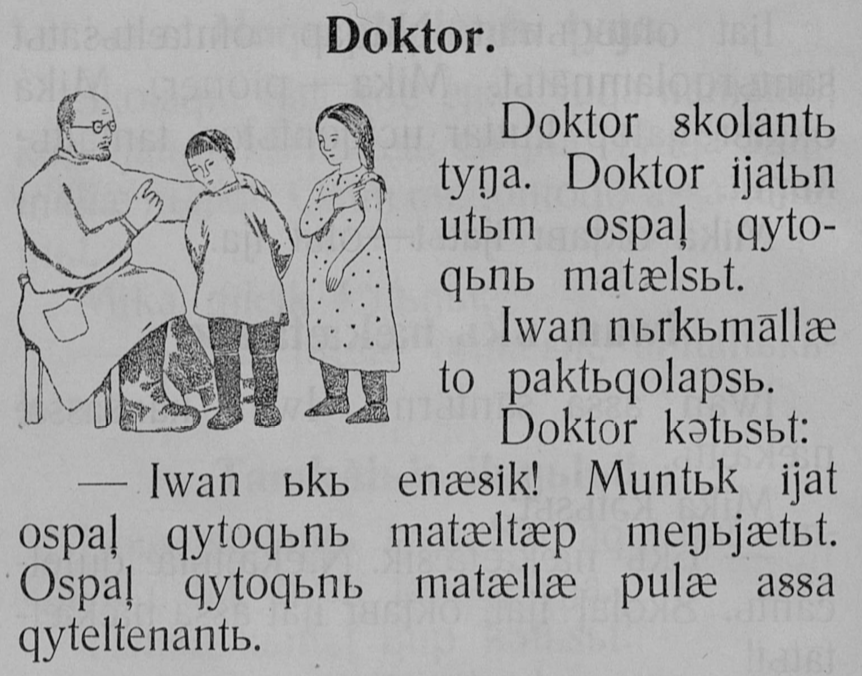
\includegraphics{images/doctor_sel.png}
\caption{Example from a book in Selkup}
\end{figure}

In Chapter \ref{tools} I go through the main tools we can currently use in OCR. Handwritten text recognition, HTR, is somewhat beyond the capabilities of this software, and in that domain \href{https://transkribus.eu/Transkribus/}{Transkribus} system has a very strong position. Thereby that is discussed separately in section \ref{htr}.

Since text recognition is closely connected to layout analysis, that is discussed in \ref{layout}. I have not personally explored much the field of layout detection, although there certainly is a lot to gain in that front. I would even say that most of our current technical problems relate to layout analysis, more than text recognition itself.

In order to start training the models, we need to acquire or create Ground Truth datasets. These are discussed, through various examples, in Chapter \ref{ground-truth}.

In the Chapter \ref{training} I finally get into actual model training, and in the Chapter \ref{using-models} I provide examples and code for using the models we trained. As will be shown, proofreading Ground Truth and training the model creates a very fast and rewarding loop, where generating more data that improves the model gets increasingly faster.

Comments, corrections and additions are more than welcome, either by email (niko.partanen@helsinki.fi), or through GitHub Issues in the project repository.

\hypertarget{tools}{%
\chapter{Tools}\label{tools}}

The OCR tools discussed here are:

\begin{itemize}
\tightlist
\item
  Ocropy
\item
  Calamari
\item
  Tesseract
\end{itemize}

I will not discuss Abbyy FineReader at length, besides saying that even though it fits well to casual use, I think it is not really the best choice for creating scientific datasets that are discussed here.

In the end of the workshop also Transkribus is discussed. It is a very exciting project that has derived impressive results on handwritten text recognition. It is very recommandable to take a look into it.

\hypertarget{layout}{%
\chapter{Layout analysis}\label{layout}}

It is important to understand that OCR systems áre primarily about working with the text content itself, traditionally at character level, but at the moment line is the normal minimum unit. The system takes a line and returns the predicted text, but it is an entirely different question how we retrieve these lines.

I would even say that OCR itself is much more a solved problem than layout detection. If we have nice lines getting out from them a relatively high accuracy text is very easy. But with complex documents a lots of work is still left in finding all the text areas, lines within them, and how all those connect together into nice running text.

Of course the argument can also be made that for variety of purposes it is not even crucial to have the lines and sections connect to one another perfectly. This could be the case, for example, in topic detection tasks etc. It is important not to fall into trap where we think that as something doesn't work perfectly we cannot use it.

Indeed, as the OCR model training does not care about anything beyond an individual line, it is not of any importance there how the lines connect to one another and whether the texts are complete.

When we use the OCR model, see section \href{./doing-ocr}{Doing OCR}, it is necessary that the lines we get from the line segmentation tool we use are similar to the lines we did the model training with. Thereby it is important to think about the whole pipeline before getting too far.

In my experience the Tesseract's layout analysis tool is very good, and often gives a very sensible result. Also Transkribus has some excellent layout detection capabilities. So running the layout detection in these programs, and extracting the line bounding boxes from the XML returned is a good option. In section \href{./doing-ocr}{Doing OCR} I also have an example of how to run the whole pipeline in Python.

\hypertarget{ground-truth}{%
\chapter{Ground Truth creation}\label{ground-truth}}

The main challenge in creating Ground Truth is that we need a comfortable environment for doing the proofreading, with safety that we know the software used will save the edited file back without any structural changes.

Lots of programmers have got the idea to build their own proofreading environment. In practice this is very complicated. Tools that allow editing beyond individual lines usually break something in the XML structure.

In principle proofreading tools / environment can be extremely simple, and this is illustrated by Ocropy in the next section.

\hypertarget{examples}{%
\section{Examples}\label{examples}}

We have training data in folders \texttt{data/batch\_1\_orig}, \texttt{data/batch\_2\_orig}, \texttt{data/batch\_3\_orig}, \texttt{data/batch\_4\_orig}, \texttt{data/batch\_5\_orig} and \texttt{data/batch\_6\_orig}. Each batch has 2 pages.

We are using Ocropy in this section, so please install Ocropy.

This is the starting position:

\begin{figure}
\centering
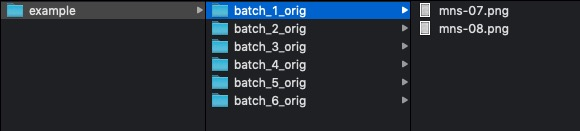
\includegraphics{./images/ocropy_starting_point.jpg}
\caption{Just scanned images}
\end{figure}

\begin{verbatim}
ocropus-nlbin ./example/batch_1_orig/*.png -o ./example/batch_1
\end{verbatim}

\begin{figure}
\centering
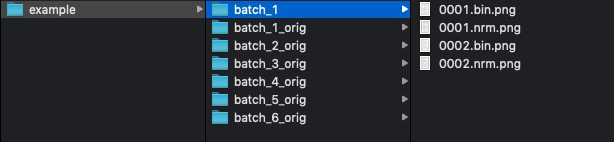
\includegraphics{./images/ocropy_binarized_pages.jpg}
\caption{Binarized pages}
\end{figure}

This tool can be used to create segmented lines. The system stores somehow information about the line locations, but moving the files around is apparently not a good idea.

\begin{verbatim}
ocropus-gpageseg ./example/batch_1/*.bin.png
\end{verbatim}

\begin{figure}
\centering
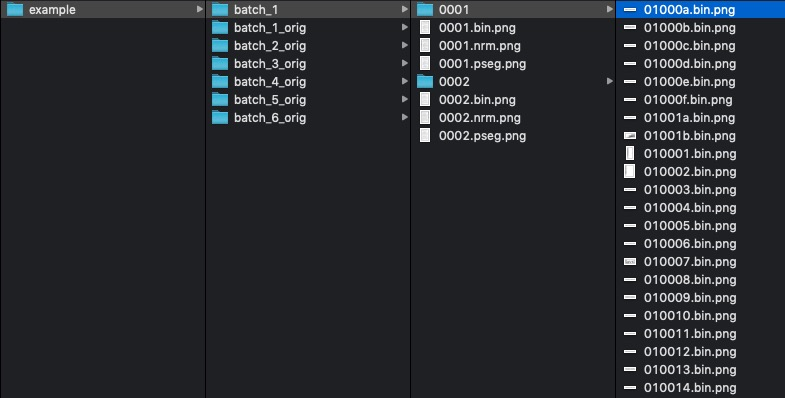
\includegraphics{./images/ocropy_segmented_lines.jpg}
\caption{Segmented lines}
\end{figure}

Now, let's pretend we are without any OCR system for this script. Then we would need to add start writing from the scratch. This could be started with the following command:

\begin{verbatim}
ocropus-gtedit html ./example/batch_1/*/*.png -o ./example/batch_1.html
\end{verbatim}

This outputs an HTML file:

\begin{figure}
\centering
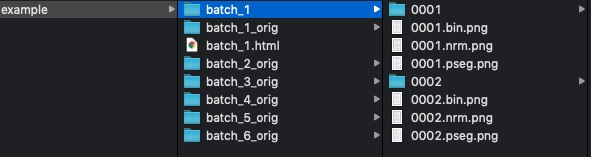
\includegraphics{./images/ocropy_created_html.jpg}
\caption{HTML file appears}
\end{figure}

\begin{figure}
\centering
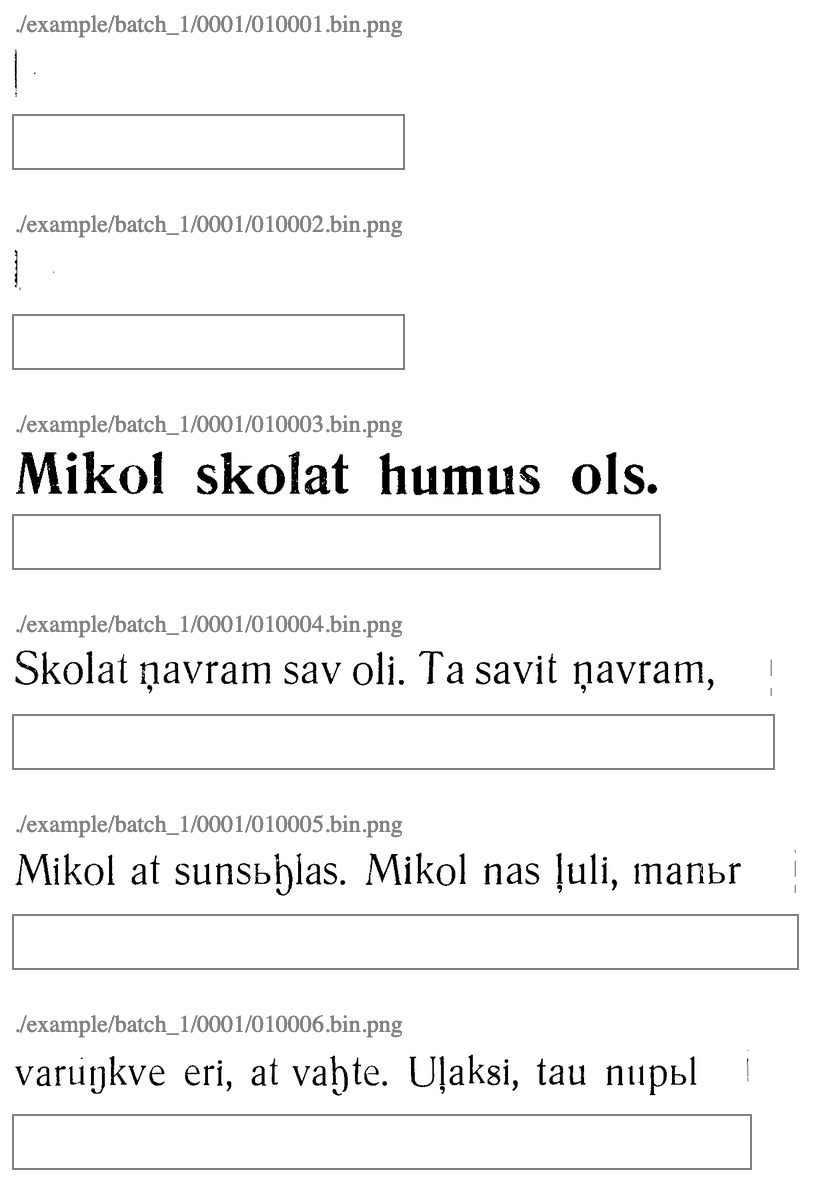
\includegraphics{./images/ocropy_empty_html.jpg}
\caption{Empty HTML from Ocropy (\textbf{has to be edited in Firefox})}
\end{figure}

However, as we have a model from an earlier work, let's use it for now.

\begin{verbatim}
ocropus-rpred -Q 4 -m ../unified-northern-alphabet-ocr/models/ocropy/mixed_model.pyrnn.gz ./example/batch_1/*/*.bin.png
\end{verbatim}

As we already see from output, the result is sensible:

\begin{verbatim}
INFO:  ./example/batch_1/0001/010003.bin.png:Mikol skolat humus ols.
INFO:  ./example/batch_1/0001/010007.bin.png:lavs:
INFO:  ./example/batch_1/0001/010004.bin.png:Skolat ņavram sav oli. Ta savit ņavram,
INFO:  ./example/batch_1/0001/010008.bin.png:- Ja! tьꜧ-unten
INFO:  ./example/batch_1/0001/010006.bin.png:varuŋkve eri, at vaꜧte. Uļakꞩi, tau nupьl
INFO:  ./example/batch_1/0001/010009.bin.png:tuŋkve patev.
INFO:  ./example/batch_1/0001/010005.bin.png:Mikol at sunsьꜧlas. Mikol nas ļuli, manьr
INFO:  ./example/batch_1/0001/01000b.bin.png:Sistamьꜧ olen.
INFO:  ./example/batch_1/0001/01000a.bin.png:Mikol, haniꞩtah-
INFO:  ./example/batch_1/0001/01000f.bin.png:- Ꞩemen luvtuŋkve eri.
INFO:  ./example/batch_1/0001/01000e.bin.png:Haniꞩtan hum lavs:
INFO:  ./example/batch_1/0001/01000c.bin.png:Ꞩemen skolan johtьs. Skolat ņavramьt
INFO:  ./example/batch_1/0001/010011.bin.png:hurataves. Puŋkane luvtuŋkve haņꞩulaves.
INFO:  ./example/batch_1/0001/01000d.bin.png:sistamьꜧ oleꜧt. Ꞩemen paŋkьŋьꜧ johtьs.
\end{verbatim}

These lines are saved with the images.

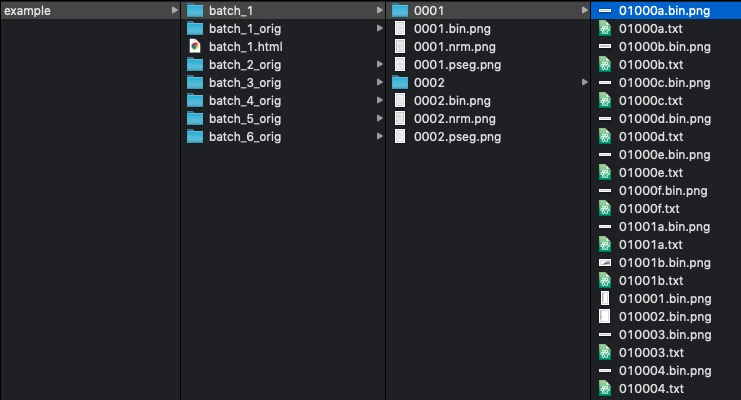
\includegraphics{./images/ocropy_export_from_html.jpg}

If we edit the HTML, and the save the file, the edited lines can be saved. This happens with:

\begin{verbatim}
ocropus-gtedit extract -O ./example/batch_1.html
\end{verbatim}

This saves the edited lines with extension \texttt{.gt.txt}.

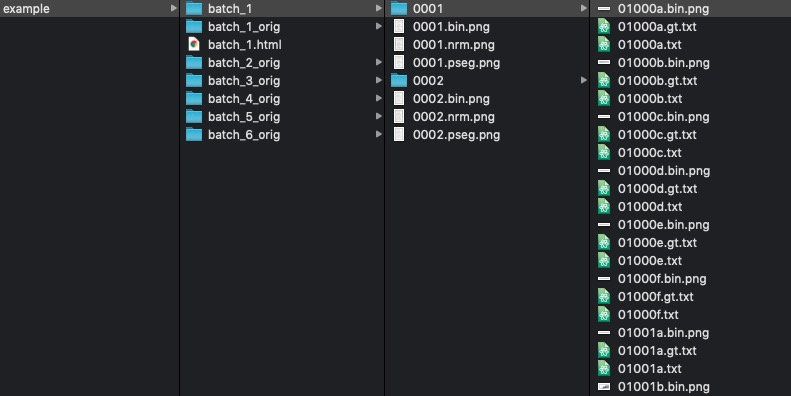
\includegraphics{./images/ocropy_export_gt.jpg}

In this point we can do:

\begin{verbatim}
cat example/batch_1/**/*gt.txt | wc -l
> 48
\end{verbatim}

More than enough! Let's go onward!

\hypertarget{summary}{%
\section{Summary}\label{summary}}

\begin{itemize}
\tightlist
\item
  \texttt{.txt} files are collected to the HTML
\item
  Proofread lines are exported from HTML
\item
  The wanted outcome is pairs of \texttt{.bin.png} and \texttt{.gt.txt} files
\item
  These can be used when training the models
\end{itemize}

The idea is that you go now to section @ref(training\} about model training, train the first model with what we have, and then the workflow described here is applied to \texttt{batch\_2}.

\hypertarget{training}{%
\chapter{OCR Model training}\label{training}}

Once we have a ground truth dataset, we can start the model training.
Most of the time this is relatively simple process, and we just run the training command and tell it where the training files are, and how we want to name the model. The system we use takes care of image preprocessing, which will then be applied also when the model is used.

There are few things we usually should keep in mind while training the model:

\begin{itemize}
\tightlist
\item
  Documenting which training files are used

  \begin{itemize}
  \tightlist
  \item
    Use Git commit hash in model name?
  \end{itemize}
\item
  Checkpoint frequency

  \begin{itemize}
  \tightlist
  \item
    Too high eats your harddisk space
  \item
    Too low is maybe difficult to monitor
  \item
    As the model accuracy can go up and down pretty wildly, it is important to notice when it is in the period of confusion, and use the model before or after that
  \end{itemize}
\item
  If you have lots of data (10,000--100,000 lines), then let it train for as long as you can

  \begin{itemize}
  \tightlist
  \item
    Same if you want to release something more publicly
  \item
    \textbf{Hot take:} With small amount of data nothing significant happens after first few hours. If you are in Ground Truth creation loop, iterating the new models fast is a good idea.
  \end{itemize}
\end{itemize}

\hypertarget{training-calamari}{%
\section{Training Calamari}\label{training-calamari}}

First, install \href{https://github.com/Calamari-OCR/calamari}{Calamari}, something like:

\begin{verbatim}
pip install calamari_ocr
pip install tensorflow 
\end{verbatim}

Or:

\begin{verbatim}
git clone https://github.com/Calamari-OCR/calamari
conda env create -f environment_master_cpu.yml
\end{verbatim}

Calamari model can be trained with a following command:

\begin{verbatim}
calamari-train --files train/*png --output_model_prefix komi-test- --output_dir models/ --checkpoint_frequency 200
\end{verbatim}

This would save the model into path \texttt{models/komi-test-000200...}. New model would be saved every 200 training steps. The models can be fairly large.

With our demo dataset there is the problem that Ocropy and Calamari prefer bit different filenames, so that Calamari doesn't want \texttt{.bin.png} ending. So let's collect the files we have into one folder, that is a nice practice anyway. I often do it with Bash like this:

\begin{verbatim}
mkdir train

for gt_line in `ls ./example/*/*/*gt.txt`

do

  bin_png=$(echo $gt_line | sed 's/gt.txt/bin.png/g')
  png=$(echo $gt_line | sed 's/gt.txt/png/g')

  cp $gt_line ./train/"${gt_line##*/}"
  cp $bin_png ./train/"${png##*/}"

done
\end{verbatim}

So we just find all Ground Truth lines, and rename + copy them into directory \texttt{train}. We could, in this point, split it into \texttt{train} and \texttt{test}, but as the data is less than 50 lines, this is maybe a bit early. It is a good idea to use tools like SciKit Learn's \texttt{train\_test\_split} in Python, but in this point it isn't that complicated what we are doing.

In the case of our demo dataset, the command would be:

\begin{verbatim}
calamari-train --files train/*png --output_model_prefix una-batch_1- --output_dir models/ --checkpoint_frequency 200

> Resolving input files
> Found 26 files in the dataset
> Preloading dataset type DataSetMode.TRAIN with size 26
> Preloading data: 100%|█████████████████████████████████████████████████████████████████████████████████████| 26/26 [00:03<00:00,  8.43it/s]
> Computing codec: 100%|██████████████████████████████████████████████████████████████████████████████████| 26/26 [00:00<00:00, 21382.73it/s]
> CODEC: ['', ' ', '!', ',', '-', '.', ':', 'A', 'H', 'M', 'O', 'P', 'S', 'T', 'U', 'a', 'e', 'g', 'h', 'i', 'j', 'k', 'l', 'm', 'n', 'o', 'p', 'r', 's', 't', 'u', 'v', 'ļ', 'Ņ', 'ņ', 'ŋ', 'ţ', 'в', 'ь', 'ꜧ', 'Ꞩ', 'ꞩ']
\end{verbatim}

Then the training starts, and what we get it something like:

\begin{verbatim}
#00000100: loss=103.64814411 ler=1.00000000 dt=1.01209140s
  PRED: '*,'
  TRUE: '*Ņavramьt tot joŋhesьt. Uļakꞩi lavs:,'
Storing checkpoint to '/Users/niko/github/ocr-tutorial/data/models/una-batch_1-00000200.ckpt'
#00000200: loss=88.01333866 ler=1.00000000 dt=1.13691821s
  PRED: '*,'
  TRUE: '*Ņavramьt tot joŋhesьt. Uļakꞩi lavs:,'
#00000300: loss=84.42394615 ler=1.00000000 dt=12.90764643s
  PRED: '*,'
  TRUE: '*vos ols.,'
Storing checkpoint to '/Users/niko/github/ocr-tutorial/data/models/una-batch_1-00000400.ckpt'
#00000400: loss=66.31870094 ler=0.88571429 dt=2.39815145s
  PRED: '*pьl ,ꜧьl jteꜧь.,'
  TRUE: '*tau nupьl lavs, aꜧmьl jemteꜧьn. Ok-,'
#00000500: loss=33.71355089 ler=0.78357143 dt=0.87875572s
  PRED: '*aki kee upьl las,'
  TRUE: '*Uļakꞩi Ꞩemen nupьl lavs:,'
Storing checkpoint to '/Users/niko/github/ocr-tutorial/data/models/una-batch_1-00000600.ckpt'
#00000600: loss=17.30537902 ler=0.68943453 dt=0.98521040s
  PRED: '*use avraьt jŋheꜧt. kol at,'
  TRUE: '*Pusen ņavramьt joŋheꜧt. Mikol at,'
WARNING:tensorflow:Method (on_train_batch_end) is slow compared to the batch update (0.302853). Check your callbacks.
#00000700: loss=9.67660141 ler=0.59846268 dt=0.94566187s
  PRED: '*Uļakꞩi pionerьꜧ oli. au okţarat sart,'
  TRUE: '*Uļakꞩi pionerьꜧ oli. Tau okţaвrat sart,'
Storing checkpoint to '/Users/niko/github/ocr-tutorial/data/models/una-batch_1-00000800.ckpt'
#00000800: loss=6.00772715 ler=0.52365484 dt=0.86985343s
  PRED: '*pьriꞩiꜧ oli.,'
  TRUE: '*pьriꞩiꜧ oli.,'
#00000900: loss=4.19488548 ler=0.47200692 dt=0.79613184s
  PRED: '*Hohsan ht-lajen, joŋhuŋkve tьꜧ-,'
  TRUE: '*- Hohsan hot-lajen, joŋhuŋkve tьꜧ-,'
Storing checkpoint to '/Users/niko/github/ocr-tutorial/data/models/una-batch_1-00001000.ckpt'
#00001000: loss=2.85367827 ler=0.42480623 dt=1.01420514s
  PRED: '*harteꜧt!,'
  TRUE: '*harteꜧt!,'
#00001100: loss=2.35952931 ler=0.39628849 dt=1.01120380s
  PRED: '*ꞩopitel.,'
  TRUE: '*ꞩopiteln.,'
Storing checkpoint to '/Users/niko/github/ocr-tutorial/data/models/una-batch_1-00001200.ckpt'
#00001200: loss=1.79808081 ler=0.36326445 dt=0.93737005s
  PRED: '*jajen.,'
  TRUE: '*jajen.,'
#00001300: loss=1.41390861 ler=0.33532103 dt=1.03504477s
  PRED: '*Ņavramьten Sano joŋhuŋkve untuves.,'
  TRUE: '*Ņavramьten Sano joŋhuŋkve untuves.,'
Storing checkpoint to '/Users/niko/github/ocr-tutorial/data/models/una-batch_1-00001400.ckpt'
#00001400: loss=1.39289295 ler=0.31136953 dt=1.04986981s
  PRED: '*Ņavramьt Uļakꞩi huntleꜧt.,'
  TRUE: '*Ņavramьt Uļakꞩi huntleꜧt.,'
#00001500: loss=0.89948882 ler=0.29061156 dt=1.21357172s
  PRED: '*vos ols.,'
  TRUE: '*vos ols.,'
Storing checkpoint to '/Users/niko/github/ocr-tutorial/data/models/una-batch_1-00001600.ckpt'
#00001600: loss=0.80192822 ler=0.27423405 dt=1.04396018s
  PRED: '*Semel part hot-osꜧeln. Hasne rakt,'
  TRUE: '*- Semel part hot-osꜧeln. Hasne rakt,'
#00001700: loss=0.76085947 ler=0.26146398 dt=1.28815659s
  PRED: '*tau nupьl lavs,aꜧmmьl jemteꜧьn. Ok-,'
  TRUE: '*tau nupьl lavs, aꜧmьl jemteꜧьn. Ok-,'
\end{verbatim}

Of course the system is only repeating the same small number of lines, so it eventually just learns them.

After having it run 2000 steps we stop, and let's test that model:

\begin{verbatim}
calamari-predict --checkpoint ./models/una-batch_1-00002000.ckpt.json --files ./mixed/*.png
\end{verbatim}

Then we test it:

\begin{verbatim}
calamari-eval --gt ./mixed/*.gt.txt
\end{verbatim}

What we get is:

\begin{verbatim}
Resolving files
Loading GT: 100%|███████████████████████████████████████████████████████████████████████████████████████| 800/800 [00:03<00:00, 250.50it/s]
Loading Prediction: 100%|███████████████████████████████████████████████████████████████████████████████| 800/800 [00:02<00:00, 329.61it/s]
Evaluation: 100%|███████████████████████████████████████████████████████████████████████████████████████| 800/800 [00:01<00:00, 552.01it/s]
Evaluation result
=================

Got mean normalized label error rate of 24.43% (5495 errs, 22494 total chars, 5585 sync errs)
GT       PRED     COUNT    PERCENT   
{ə}      {a}           237      4.24%
{d}      {ol}          195      6.98%
{m}      {n}           153      2.74%
{n}      {}            133      2.38%
{m}      {nn}           98      3.51%
{w}      {v}            90      1.61%
{æ}      {ae}           85      3.04%
{q}      {op}           82      2.94%
{ļ}      {}             80      1.43%
{c}      {o}            73      1.31%
The remaining but hidden errors make up 69.81%
\end{verbatim}

Error rate of 24.43\% means that every fourth character needs to be fixed, but that is already much better than what we had in the beginning.

\hypertarget{training-tesseract}{%
\section{Training Tesseract}\label{training-tesseract}}

Training Tesseract can be a bit intimidating process. In last years many improvements have been done, and at the moment training is possible on both Linux and Mac. There is, additionally, \href{https://github.com/tesseract-ocr/tesstrain}{tessmake} project that very conveniently wraps the training process into a Makefile.

\begin{verbatim}
make training MODEL_NAME=komi-test GROUND_TRUTH_DIR=train/
\end{verbatim}

If you want to change the parameters, play around with the Makefile.

This gives a very good Tesseract model if you have enough data. The models, to be foundable for Tesseract, have to be in so called tessdata directory. This can be also specified when using Tesseract by specifying \texttt{-\/-tessdata-dir}.

\hypertarget{htr}{%
\chapter{Handwritten text recognition}\label{htr}}

At the moment \href{https://transkribus.eu}{Transkribus} project offers the best platform for handwritten text recognition, as well as for lots of OCR related tasks. Training also OCR models with the Transkribus system seems to work extremely, even ridiculously, well, so that is certainly worth playing around.

One example of how collections edited in Transkribus can be made available can be seen in this interface for \href{https://transkribus.eu/r/kansallisarkisto/}{National Archives of Finland}'s data.

\hypertarget{using-models}{%
\chapter{Using OCR models}\label{using-models}}

In this section we go through with practical examples how OCR models can be used.chr

\hypertarget{using-tesseract}{%
\section{Using Tesseract}\label{using-tesseract}}

Tesseract\ldots{}

R bindings\ldots{}

Python bindings\ldots{}

\hypertarget{using-calamari}{%
\section{Using Calamari}\label{using-calamari}}

Calamari\ldots{}

\bibliography{book.bib,packages.bib,bibtex/FRibliography.bib}


\end{document}
